%
%	PREÁMBULO DEL DOCUMENTO
%



%
%	Inicio del documento. Aquí declaramos la clase del archivo.
%
\documentclass[a4paper]{article}


% Hace que podamos escribir directamente con tildes y acentos en el documento.
\usepackage{fontspec}


% Adecuación a la tipografía y silabación del español.
\usepackage{polyglossia}
\setmainlanguage{spanish}


% Añade márgenes más pequeños al documento debido a que los que están por defecto son muy generosos.
\usepackage[left=20mm,right=20mm,top=20mm,bottom=20mm]{geometry}


% Permite la carga de imágenes en formatos jpeg, png, svg y pdf.
\usepackage{graphicx}

% Añade el colocador H a los elementos deslizantes
\usepackage{float}

% Crea hipervínculos entre las referencias y etiquetas que se hayan escrito.
\usepackage{hyperref}


% Paquetes de utilidad matemática
\usepackage{amsmath}
\usepackage{amsfonts}
\usepackage{amssymb}


% Parámetros que queremos que estén en el título

\title{Un ejemplo de cómo funciona \LaTeX}
\author{Ismael Aderdor \\ <ikabliz@asaaf.org>}
\date{3 de abril de 2017}

%
%	CUERPO DEL DOCUMENTO
%

\begin{document}

% Crea el título
\maketitle

% Crea el índice de contenidos
\tableofcontents



% Comienza una sección. Es recomendable dejar un poco de espacio arriba y abajo para identificarlas más rápido.
\section{Inicio}
\label{Sec:inicio}	% Etiqueta que para hacer referencias a la sección.


Lorem ipsum dolor sit amet, consectetur adipiscing elit. Etiam vel diam ut felis posuere commodo eu ut dolor. Pellentesque eu accumsan ex, ac luctus massa. Nulla sit amet nulla auctor, condimentum mauris in, sollicitudin neque. Vestibulum ullamcorper id lacus non ullamcorper. Curabitur pharetra pretium mauris ut venenatis. Cras eget volutpat erat. Quisque interdum diam eu nibh porttitor finibus. Orci varius natoque penatibus et magnis dis parturient montes, nascetur ridiculus mus. Fusce sed pellentesque ipsum. Class aptent taciti sociosqu ad litora torquent per conubia nostra, per inceptos himenaeos. Sed sit amet metus ac leo ultricies mattis. Duis dictum sagittis nisl ac placerat. Ut elementum quis erat viverra dapibus.



\subsection{Teorema interesante}


Nunc vehicula aliquet risus, sed hendrerit leo suscipit eget. Phasellus ultrices mattis laoreet. Fusce porta lacus et massa fringilla, nec porta sem convallis. Ut finibus eu est in rhoncus. Morbi viverra massa id nibh porttitor, sed ullamcorper metus gravida. Integer at eleifend orci, vel lacinia lorem. Phasellus vitae nisi ipsum.


% Aquí definimos un elemento deslizante que queremos que sitúe exactamente aquí. El elemento contiene una tabla.
\begin{figure}[H]
	\centering
	\begin{tabular}{ccc}
	Nombre & Puntos & Tiempo \\ 
	Minkowski & 25pts & 3h 45m 
	\end{tabular}
\end{figure}


Sed commodo porttitor mauris. Cras venenatis enim sit amet sagittis volutpat. Morbi in interdum nunc, ac sagittis arcu. Mauris at mi gravida, sodales est eu, auctor sapien. Duis vulputate ac erat id pharetra. Maecenas ac interdum mi. Donec nulla sapien, mollis sed sapien eu, malesuada vulputate est. In vitae vulputate augue.



\section{Segunda sección}


Vestibulum ut dui ipsum. Integer euismod euismod mauris a facilisis. Vivamus commodo nibh libero, semper gravida tellus vulputate sit amet. Quisque ut fermentum mi. Etiam efficitur euismod turpis. Suspendisse potenti. Suspendisse non bibendum ipsum, consequat lacinia tellus. Sed rhoncus tincidunt orci quis consectetur. Maecenas quis rhoncus risus. Ut arcu risus, varius sit amet magna quis, imperdiet aliquet erat.


% Aquí estamos definiendo un elemento deslizante que contiene una imagen.
\begin{figure}[H]
	\centering
	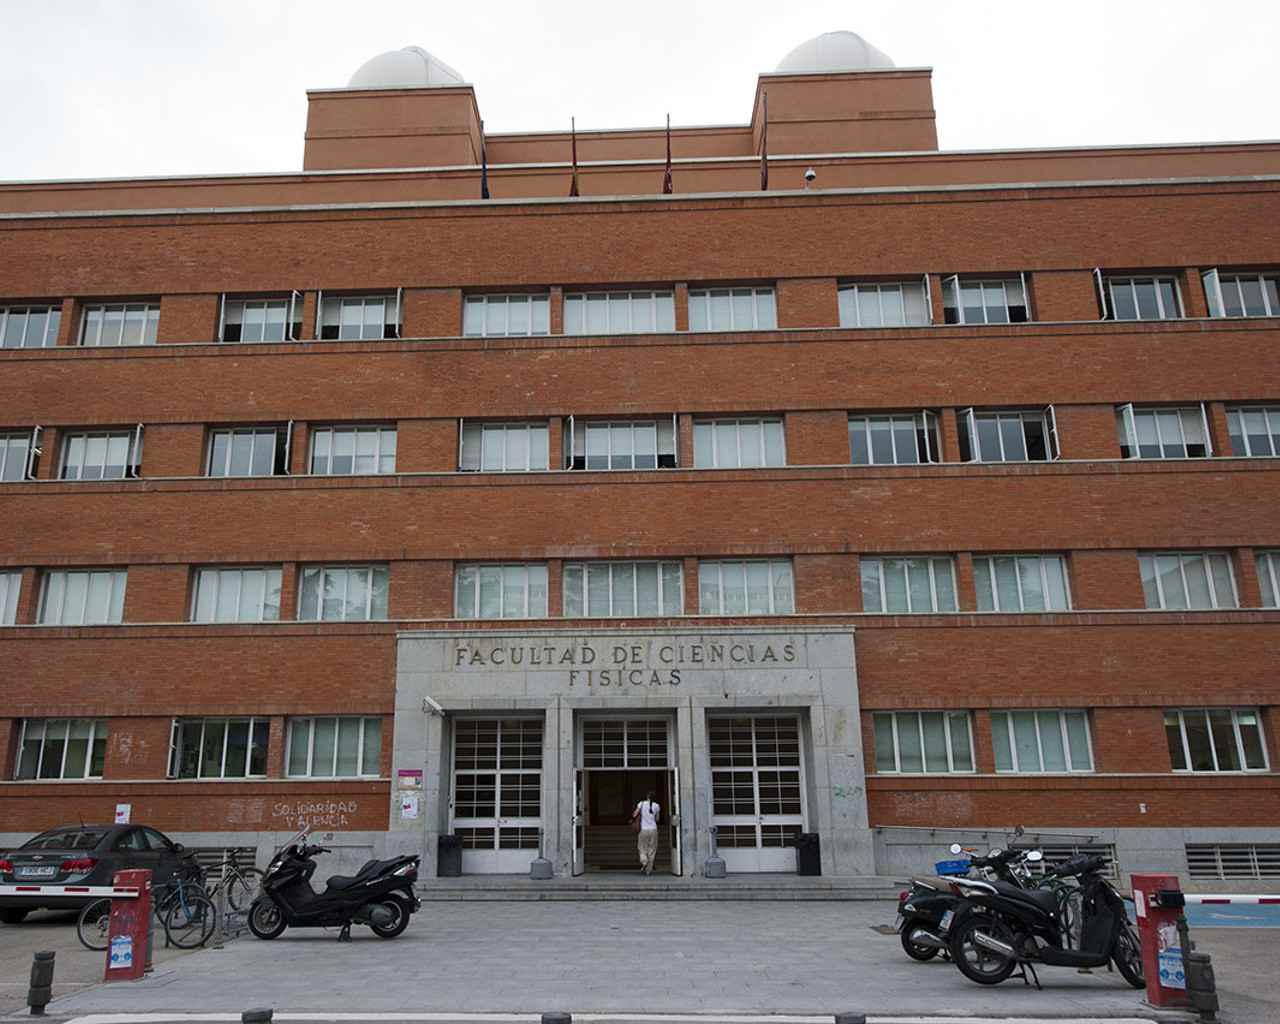
\includegraphics[scale=.3]{img/imagen}	% No he añadido
	\caption{Una fotografía de la entrada de la Facultad de Ciencias Físicas de la UCM.}
	\label{fig:patio}
\end{figure}



Ut nec purus aliquam metus auctor malesuada eget et massa. Donec nec est eleifend, sagittis enim et, pharetra magna. Aenean facilisis augue vitae arcu condimentum, sit amet aliquet erat ullamcorper. Sed ornare risus sit amet lacinia ultricies. Sed id hendrerit metus, eget interdum felis. Interdum et malesuada fames ac ante ipsum primis in faucibus. Pellentesque facilisis sodales nunc sit amet euismod. Donec interdum ut neque ut pretium. Sed vel sodales quam.

% En este párrafo hemos hecho una referencia a la primera sección.
Referencia a la sección \ref{Sec:inicio}.



% Aquí hemos definido una sección que no se indexará ni se numerará.
\section*{Bibliografía}


Fusce porta velit imperdiet elit interdum, ac bibendum purus porta. Nunc ante odio, faucibus sed tincidunt vulputate, egestas aliquet felis. Sed mollis condimentum ex, sit amet consequat elit tempus non. Suspendisse a nunc in massa bibendum tempor. Morbi elementum quam libero, vitae euismod massa volutpat at.

% Esto es una ecuación "en línea".
Suspendisse non arcu $\sum_i ^n x_i$ sit amet mauris tempus lobortis et sit amet sapien. 

% Aquí va una ecuación "destacada". Nótese que está numerada.
\begin{equation}
	E = mc^2
\end{equation}


% Esto es un ejemplo de una ecuación "destacada" sin numerar.
\[
	\nabla \cdot %
	\vec{ B } = 0
\]



\end{document}